\documentclass{article}
\usepackage[latin1]{inputenc}
\usepackage{graphicx}
\usepackage{a4wide}

\title{Micro Helicopter API: analysis}
\author{Cedric Pradalier}
\begin{document}
\maketitle

\section{Introduction}
\label{sec:intro}
This document provides a first analysis of an API for an easy to use
micro-helicopter. It is intended as a discussion document. No conclusions are
definitive, everything is arguable. 

Most important, this has been written from a user point of view: it shows what
I think a user would expect, without taking into account the reality of the
controller implementation. 

\section{Modes}
\label{sec:modes}
\begin{figure}[htb]
\centering
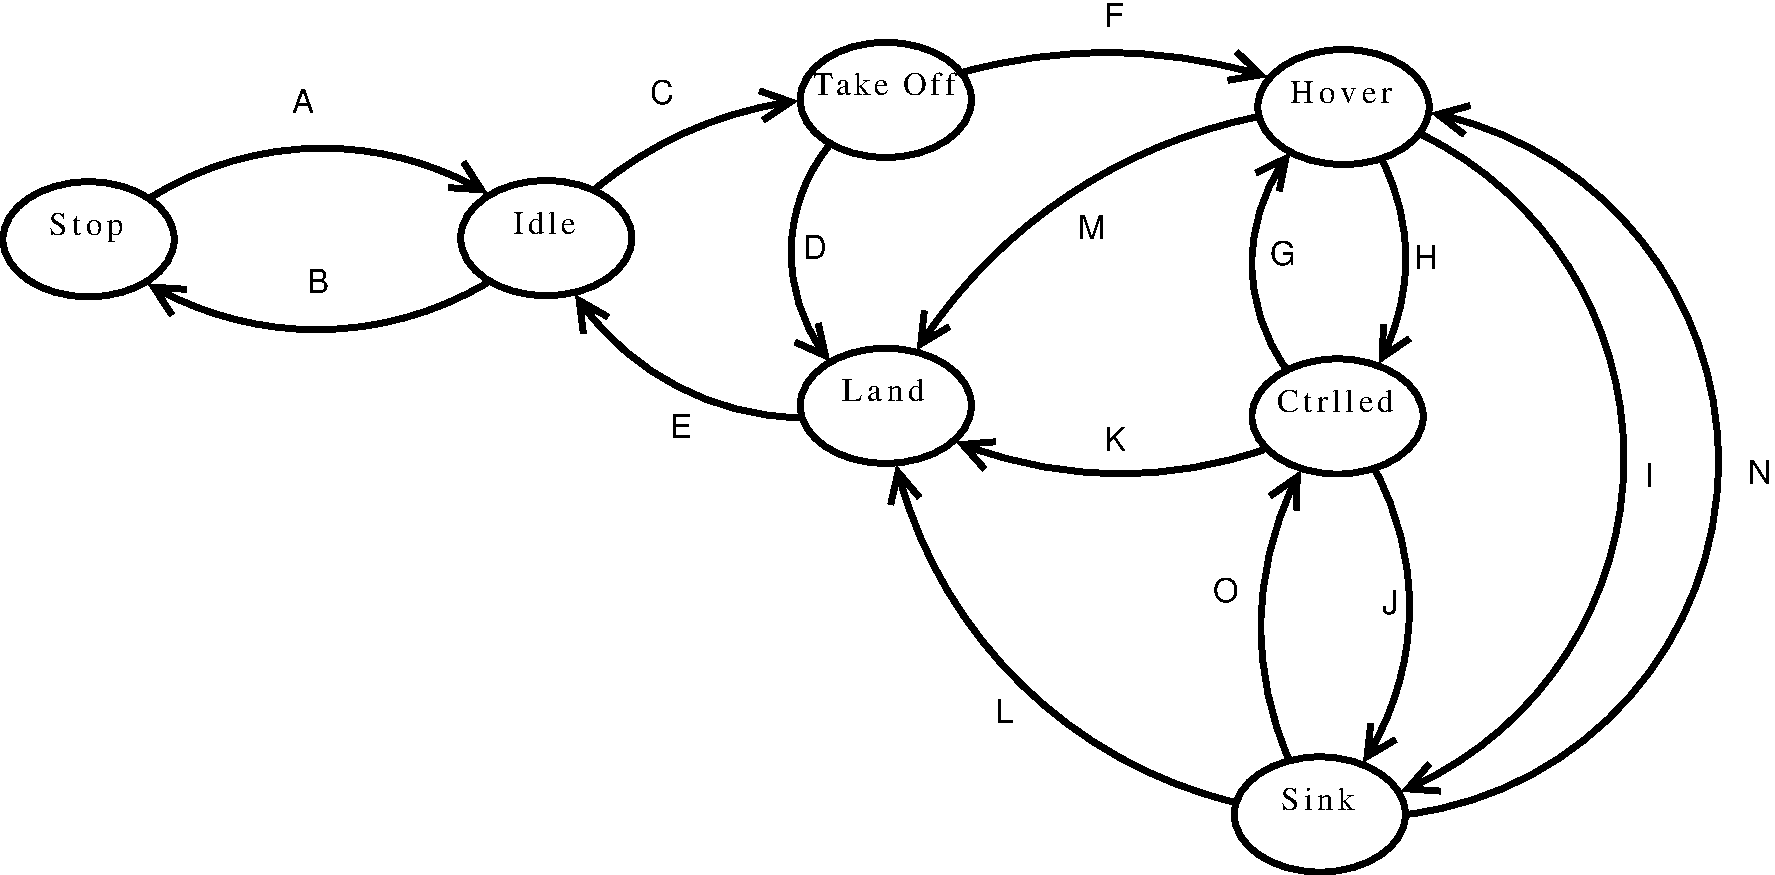
\includegraphics[width=0.9\columnwidth]{API_automaton}
\caption{MAV API: Envisaged control modes}
\label{fig:automaton}
\end{figure}
Figure \ref{fig:automaton} is a state automaton showing the various behaviour
modes expected from a MAV. It is important to notice that these modes may be
virtual modes: they don't have to correspond to what is really implemented in
the controller, they describes various behaviours, semantically consistent and
with the same set of constraints. The remaining of this section details the
expected behaviour in each mode, the transition conditions and the accepted
commands.

For the safety of the MAV, it is assumed that a control watchdog is
implemented. This watchdog is triggered when the connection between the MAV and
the host computer is broken, or if the host controller stop sending control
commands. See section \ref{sec:usecases} for details.

\subsection{Stop}
\subsubsection{Description}
\begin{itemize}
\item System is checked up
\item All the motors are powered off
\item The pressure sensor reference is initialised
\end{itemize}
\subsubsection{Transition conditions}
\begin{description}
\item[Transition A]: on user request.
\end{description}
\subsubsection{Accepted commands}
\begin{itemize}
\item Set Mode to Idle
\end{itemize}

\subsection{Idle}
\subsubsection{Description}
\begin{itemize}
\item All systems powered on
\item All motors rotating slowly
\end{itemize}
\subsubsection{Transition conditions}
\begin{description}
\item[Transition B]: on user request or on watchdog timeout
\item[Transition C]: on user request: mode set to Take Off or Hover
\end{description}
\subsubsection{Accepted commands}
\begin{itemize}
\item Set Mode to Stop, Take Off or Hover
\end{itemize}

\subsection{Take Off}
\subsubsection{Description}
\begin{itemize}
\item The MAV stabilise itself to hovering at 10cm above ground (TBC), based on
pressure sensor. The resulting displacement is relative.
\end{itemize}
\subsubsection{Transition conditions}
\begin{description}
\item[Transition F]: the system is stable at the required height.
\item[Transition D]: on user request, watchdog timeout, action timeout or exception.
\end{description}
\subsubsection{Accepted commands}
\begin{itemize}
\item Set Mode to Land
\end{itemize}

\subsection{Land}
\subsubsection{Description}
\begin{itemize}
\item Bring the MAV to touch down. Downward range sensor is used to estimate
touch down. The maximum velocity downward is XX (TBD). 
\end{itemize}
\subsubsection{Transition conditions}
\begin{description}
\item[Transition E]: Contact has been detected.
\end{description}
\subsubsection{Accepted commands}
\begin{itemize}
\item None
\end{itemize}

\subsection{Hover}
\subsubsection{Description}
\begin{itemize}
\item Yaw and altitude are kept constant, roll and pitch kept to zero. The MAV
will certainly be drifting in this mode.
\item If available, the horizontal obstacle avoidance is active.
\item Downward obstacle avoidance is active
\item Data fusion for altitude estimation is active. 
\end{itemize}
\subsubsection{Transition conditions}
\begin{description}
\item[Transition H]: on user request
\item[Transition I]: on watchdog timeout
\item[Transition M]: on user request
\end{description}
\subsubsection{Accepted commands}
\begin{itemize}
\item Set Mode to Land
\item Set Mode to Controlled
\end{itemize}

\subsection{Controlled -- Ctrlled}
\subsubsection{Description}
\begin{itemize}
\item Altitude, yaw and position are controlled as requested
\item Downward obstacle avoidance may be activated
\item If available, horizontal obstacle avoidance may be activated
\end{itemize}
\subsubsection{Transition conditions}
\begin{description}
\item[Transition G]: on user request or on control timeout (i.e. the watchdog
has not been triggered, but no remote commands have been received).
\item[Transition J]: on watchdog timeout 
\item[Transition K]: on user request
\end{description}
\subsubsection{Accepted commands}
\begin{itemize}
\item Set Mode to Hover
\item Set Mode to Land
\item Desired altitude, yaw and horizontal controls. In position or rate as
available. 
\end{itemize}

\subsection{Sink}
\subsubsection{Description}
\begin{itemize}
\item Altitude is slowly controlled down (for instance 5cm/s) until touch down
\item Any desired control is ignored until the connection is reset (see section
\item If available, the horizontal obstacle avoidance is active.
\ref{sec:functions}).
\end{itemize}
\subsubsection{Transition conditions}
\begin{description}
\item[Transition N]: on user request after connection reset.
\item[Transition O]: on user request after connection reset.
\item[Transition L]: on user request after connection reset, or when the
distance to ground becomes smaller than 10cm (TBC).
\end{description}
\subsubsection{Accepted commands}
\begin{itemize}
\item Set Mode to Hover
\item Set Mode to Land
\item Set Mode to Controlled
\end{itemize}


\newpage
\section{Use Cases: from the programmer side}
\label{sec:usecases}
Several type of user programming can be foreseen. This section try to list them
all. Not all of them may be implementable.

\subsection{Considering only one helicopter}
\subsubsection{Polling, single thread}
\begin{tabbing}
\=\hspace{1cm}\=\hspace{6cm}\=\kill
Set Communication Mode to Polling\\
\>Forever:\\
\>\>Get MAV State\>{\it Polling}\\
\>\>Set Control Mode\>{\it Reset WatchDog}\\
\>\>Set Control \>{\it Z, Yaw, ...}
\end{tabbing}

\subsubsection{Polling, multi thread}
Set Communication Mode to Polling\\
\begin{tabular}{|l|l|}
\hline
Thread 1 & Thread 2 \\
\hline
\begin{minipage}{0.49\columnwidth}
\vspace{2mm}
Forever:\\
\hspace*{1cm}Get MAV State \\
\vspace{2mm}
\end{minipage} &
\begin{minipage}{0.49\columnwidth}
\vspace{2mm}
Forever:\\
\hspace*{1cm}Set Control Mode\\
\hspace*{1cm}Set Control\\
\vspace{2mm}
\end{minipage} \\
\hline
\end{tabular}

\subsubsection{Continuous, single thread}
\begin{tabbing}
\=\hspace{1cm}\=\hspace{6cm}\=\kill
\>Set Communication Mode to Continuous\\
\>Forever:\\
\>\>Receive MAV State\>{\it Server push}\\
\>\>Set Control Mode\>{\it Reset WatchDog}\\
\>\>Set Control \>{\it Z, Yaw, ...}
\end{tabbing}

\subsubsection{Continuous, multi thread}
Set Communication Mode to Continuous\\
\begin{tabular}{|l|l|}
\hline
Thread 1 & Thread 2 \\
\hline
\begin{minipage}{0.49\columnwidth}
\vspace{2mm}
Forever:\\
\hspace*{1cm}Receive MAV State \\
\vspace{2mm}
\end{minipage} &
\begin{minipage}{0.49\columnwidth}
\vspace{2mm}
Forever:\\
\hspace{1cm}Set Control Mode\\
\hspace*{1cm}Set Control\\
\vspace*{2mm}
\end{minipage} \\
\hline
\end{tabular}

\subsubsection{The video}
In addition to the above options, the video stream can also be polled or
received continuously, and it could (or should) be acquired in an independent
thread. 

\subsection{Considering several helicopter}
The type of MAV developed by SkyBotics are likely to be very suitable for
multi-UAV control. This should be taken into account when designing the API, so
that multiple UAV can be controlled from a single host computer. 

\newpage
\section{Identified functions}
\label{sec:functions}
Based on the above use cases, the following functions have been identified.
They should all be implemented in a thread-safe manner. If not possible, it is
always possible to specify that the user has to protect them appropriately.

\subsection{System}
\subsubsection{Connect(MAV\_id, Observer:bool)}
\begin{itemize}
\item Connects to the MAV "MAV\_id" as a controller or as a simple observer.
\item Returns a handle describing the connection. 
\end{itemize}
The assumption behind this function is that the MAV can only have one
controller. On the other hand, we can design so has to allow multiple observer.
Furthermore, after a timeout or an error in the communication, the
communication must be reset before accepting new control. This can prevent
chattering in case of a process too slow to control the MAV properly. 

Each time a connection request is received, the connection id is increased by
1. As a result, a connection id can be 
\begin{itemize}
\item Active: it is the id of the host controller currently controlling the MAV
\item Inactive: it is not yet a valid id
\item Revoked: it was a valid id, but has been revoked due to a disconnection
or a timeout
\item Observer: it is the id of an observer, probably 0 (TBC)
\end{itemize}

The resulting handle is composed on the MAV\_id and the connection id.

The communication channel is currently expected to be Bluetooth.

\subsubsection{Disconnect(handle)}
\begin{itemize}
\item Close the connection and revoke the connection id
\item No return
\end{itemize}

\subsubsection{HasVideo(handle)}
\begin{itemize}
\item Test if a video stream is installed on this MAV
\item Bool
\end{itemize}

\subsubsection{SetObstacleAvoidance(handle,vertical,horizontal)}
\begin{itemize}
\item Enable or disable the obstacle avoidance control in vertical or
horizontal direction if available.
\item No return
\end{itemize}

\subsubsection{SetCommunicationMode(handle,mode)}
\begin{itemize}
\item Set the communication mode to polling or continuous
\item No return
\end{itemize}
In polling mode, the MAV state is sent to the host controller only on request.
In continuous mode, the MAV controller keeps pushing data to the host
controller. The latter is responsible for collecting these data fast enough to
keep the channel clear. Failure to do so should provoke a timeout and revoke
the connection id.

The expected data rate is 50Hz, in polling or continuous mode.

See also GetState and ReceiveState functions

\subsection{Video System}

\subsubsection{ConnectVideo(handle, ip)}
\begin{itemize}
\item Open a connection to the MAV embedded computer so as to stream video
data.
\item Returns a handle on the video connection
\end{itemize}
The assumption here is that the embedded computer is accessible via a wireless
lan on the given ip. The TCP/IP layer of the embedded computer will be used to
stream the video frame.

\subsubsection{DisconnectVideo(handle)}
\begin{itemize}
\item Close the connection 
\item No return
\end{itemize}

\subsubsection{SetVideoCommunicationMode(handle,mode)}
\begin{itemize}
\item Set the video streaming mode to polling or continuous
\item No return
\end{itemize}
In polling mode, the video frames are sent only on request.
In continuous mode, the MAV embedded computer keeps pushing data to the host
controller. The latter is responsible for collecting these data fast enough to
keep the channel clear. Failure to do so should provoke a timeout and close the
connection.

\subsection{Data Collection}
\subsubsection{GetState(handle)}
\begin{itemize}
\item Request the state of the MAV, only valid in polling mode
\item Returns a structure describing the state as follows:
\begin{itemize}
\item timeStamp:
\item handleState: Active, Inactive, Revoked, Timedout
\item commMode: Polling, Continuous
\item mavMode: id of an automaton state from section \ref{sec:modes}.
\item obstacleAvoidanceMode [vertical horizontal]
\item axisMode: control mode of the axis, see SetAxisMode.
\item errorFlags: TBD
\item Roll, Pitch, Yaw: from the IMU
\item Roll rate, Pitch rate, Yaw rate: from the IMU if available
\item Z, (Zrate if available): fused altitude estimation
\item Pressure
\item Battery
\item Proximeter [Down Left, Right, Front, Back]
\item RPM if available
\end{itemize}
\end{itemize}

\subsubsection{ReceiveState(handle)}
\begin{itemize}
\item Wait to receive the state of the MAV, only valid in continuous mode
\item Returns a structure describing the state as GetState
\end{itemize}

\subsubsection{GetVideo(vhandle)}
\begin{itemize}
\item Request a video frame, only valid in video polling mode
\item Returns the video frame, in a format to be specified.
\end{itemize}

\subsubsection{ReceiveVideo(vhandle)}
\begin{itemize}
\item Wait to receive the next video frame, only valid in video continuous mode
\item Returns the video frame, in a format to be specified.
\end{itemize}

\subsection{Control}
\subsubsection{SetMode(handle,mode)}
\begin{itemize}
\item {\bf Reset the WatchDog timer}
\item Change the control mode as specified in the automaton in section
\ref{sec:modes}. If the requested mode change is invalid in this context, it is
ignored.
\item Returns a flag indicating if the mode was accepted
\end{itemize}
The idea behind this function is that any user program should continuously call
it to confirm its intention to take charge of the MAV. If not called at a high
enough frequency, the MAV will slowly touch down, land and stop the rotors. 

The watchdog function could also be an independent function, similar to the
Pulse function on pioneers. TBD.

\subsubsection{SetAxisMode(handle,yaw,altitude,horizontal)}
\begin{itemize}
\item Defines the control mode of for each independent axis. Each control mode
can be PositionControl or RateControl. Some of them may not be applicable
currently and shall be ignored. 
\item Returns an acknowledgement
\end{itemize}
The expected default for the MAV control are:
\begin{itemize}
\item Yaw: position control, rate available
\item Altitude: position control, rate available
\item Horizontal: open loop rate control
\end{itemize}

\subsubsection{SetControl(handle, yaw, altitude, horizontal}
\begin{itemize}
\item In Controlled mode, set the desired yaw, altitude and horizontal control.
The resulting control is affected by the AxisMode
\item Returns an acknowledgement
\end{itemize}


\end{document}

